% answers.tex —— 1977 年·江苏常州市初试卷 · 参考答案与详细解析片段
% 由 tools/generate_projects.py 依来源总账自 1977/1977_数学真题_江苏常州市初试_试题.md + 1977/1977_数学真题_江苏常州市初试_解析正文.md + 1977/1977_数学真题_江苏常州市初试_答案要点.md 生成，勿手改（改源 MD 后重跑）


\begin{gktip}
固定源为纯题面扫描件（初试题汇编「二、常州市」部分，共 3 页，未附解答）。以下逐题独立推导；原卷各题小问编号连续，无跳号处理。第 13 题按原卷随题附印的反对数表（标准四位反对数表第 80—84 行节选）完成查表计算。
\end{gktip}

\begin{answer}
\gksolhead{1}{}

\textbf{题目}（7 分）：

\Needspace{5\baselineskip}
计算：

\nopagebreak[4]
\[
-1-\left(-5\frac{1}{2}\right)\times\frac{4}{11}+(-2)^3\div\left[(-3)^2+7\right].
\]

\Needspace{4\baselineskip}
\textbf{解析}

\Needspace{5\baselineskip}
按运算顺序先算乘方与括号：

\nopagebreak[4]
\[
\left(-5\frac{1}{2}\right)\times\frac{4}{11}=-\frac{11}{2}\times\frac{4}{11}=-2,
\]

\nopagebreak[4]
\[
(-2)^3\div\left[(-3)^2+7\right]=-8\div(9+7)=-\frac{1}{2}.
\]

\Needspace{5\baselineskip}
所以

\nopagebreak[4]
\[
-1-(-2)+\left(-\frac{1}{2}\right)=-1+2-\frac{1}{2}=\frac{1}{2}.
\]

\gkanswer{答案：$\dfrac{1}{2}$。}

\end{answer}
\begin{answer}
\gksolhead{2}{}

\textbf{题目}（7 分）：

\Needspace{5\baselineskip}
计算：

\nopagebreak[4]
\[
\frac{2}{2+\sqrt{2}}+\frac{1}{\sqrt{3}-\sqrt{2}}-\frac{3+\sqrt{3}}{3-\sqrt{3}}.
\]

\Needspace{4\baselineskip}
\textbf{解析}

\Needspace{5\baselineskip}
三分母分别有理化：

\nopagebreak[4]
\[
\frac{2}{2+\sqrt{2}}=\frac{2(2-\sqrt{2})}{(2+\sqrt{2})(2-\sqrt{2})}=\frac{4-2\sqrt{2}}{2}=2-\sqrt{2},
\]

\nopagebreak[4]
\[
\frac{1}{\sqrt{3}-\sqrt{2}}=\sqrt{3}+\sqrt{2},
\]

\nopagebreak[4]
\[
\frac{3+\sqrt{3}}{3-\sqrt{3}}=\frac{(3+\sqrt{3})^2}{(3+\sqrt{3})(3-\sqrt{3})}=\frac{12+6\sqrt{3}}{6}=2+\sqrt{3}.
\]

\Needspace{5\baselineskip}
于是原式

\nopagebreak[4]
\[
(2-\sqrt{2})+(\sqrt{3}+\sqrt{2})-(2+\sqrt{3})=0.
\]

\gkanswer{答案：$0$。}

\end{answer}
\begin{answer}
\gksolhead{3}{}

\textbf{题目}（6 分）：

计算：$\log_2(1+\lg10)$。

\Needspace{4\baselineskip}
\textbf{解析}

\Needspace{5\baselineskip}
由 $\lg10=1$，得

\nopagebreak[4]
\[
\log_2(1+\lg10)=\log_2 2=1.
\]

\gkanswer{答案：$1$。}

\end{answer}
\begin{answer}
\gksolhead{4}{}

\textbf{题目}（8 分）：

$\sin390^\circ\cos(-60^\circ)+\sin120^\circ\cos750^\circ.$

\Needspace{4\baselineskip}
\textbf{解析}

\Needspace{5\baselineskip}
用诱导公式化简各项：

\nopagebreak[4]
\[
\sin390^\circ=\sin30^\circ=\frac{1}{2},\qquad
\cos(-60^\circ)=\cos60^\circ=\frac{1}{2},
\]

\nopagebreak[4]
\[
\sin120^\circ=\sin60^\circ=\frac{\sqrt{3}}{2},\qquad
\cos750^\circ=\cos(2\times360^\circ+30^\circ)=\cos30^\circ=\frac{\sqrt{3}}{2}.
\]

\Needspace{5\baselineskip}
所以

\nopagebreak[4]
\[
\sin390^\circ\cos(-60^\circ)+\sin120^\circ\cos750^\circ
=\frac{1}{2}\times\frac{1}{2}+\frac{\sqrt{3}}{2}\times\frac{\sqrt{3}}{2}
=\frac{1}{4}+\frac{3}{4}=1.
\]

\gkanswer{答案：$1$。}

\end{answer}
\begin{answer}
\gksolhead{5}{}

\textbf{题目}（8 分）：

化简：$a+\sqrt{a^2-2a+1}$。

\Needspace{4\baselineskip}
\textbf{解析}

\nopagebreak[4]
\[
a+\sqrt{a^2-2a+1}=a+\sqrt{(a-1)^2}=a+|a-1|.
\]

原卷未给出 $a$ 的取值范围，按绝对值分情况：

\begin{itemize}
\item 当 $a\ge1$ 时，原式 $=a+(a-1)=2a-1$；
\item 当 $a<1$ 时，原式 $=a+(1-a)=1$。
\end{itemize}

\gkanswer{答案：当 $a\ge1$ 时为 $2a-1$；当 $a<1$ 时为 $1$。}

\end{answer}
\begin{answer}
\gksolhead{6}{}

\textbf{题目}（8 分）：

\Needspace{5\baselineskip}
已知 $a=9$，$b=\sqrt{3}$，求

\nopagebreak[4]
\[
a^{\frac{3}{2}}b\left(\frac{b^2}{a}\right)^{\frac{1}{2}}\div\left(\frac{1}{a}\right)^{-\frac{1}{2}}
\]

的值。

\Needspace{4\baselineskip}
\textbf{解析}

\Needspace{5\baselineskip}
代入 $a=9$、$b=\sqrt{3}$，逐项计算：

\nopagebreak[4]
\[
a^{\frac{3}{2}}=9^{\frac{3}{2}}=(\sqrt{9})^3=27,
\]

\nopagebreak[4]
\[
\left(\frac{b^2}{a}\right)^{\frac{1}{2}}=\left(\frac{3}{9}\right)^{\frac{1}{2}}=\left(\frac{1}{3}\right)^{\frac{1}{2}}=\frac{1}{\sqrt{3}},
\qquad
\left(\frac{1}{a}\right)^{-\frac{1}{2}}=\left(\frac{1}{9}\right)^{-\frac{1}{2}}=9^{\frac{1}{2}}=3.
\]

\Needspace{5\baselineskip}
所以

\nopagebreak[4]
\[
27\times\sqrt{3}\times\frac{1}{\sqrt{3}}\div3=27\div3=9.
\]

\gkanswer{答案：$9$。}

\end{answer}
\begin{answer}
\gksolhead{7}{}

\textbf{题目}（8 分）：

求函数 $y=\sqrt{x-3}+\sqrt{5-x}$ 的自变量的取值范围。

\Needspace{4\baselineskip}
\textbf{解析}

\Needspace{5\baselineskip}
两个根号内的式子都须非负：

\nopagebreak[4]
\[
\begin{cases}
x-3\ge0,\\
5-x\ge0,
\end{cases}
\quad\Longrightarrow\quad
3\le x\le5.
\]

\gkanswer{答案：$3\le x\le5$。}

\end{answer}
\begin{answer}
\gksolhead{8}{}

\textbf{题目}（8 分）：

\Needspace{5\baselineskip}
求证：

\nopagebreak[4]
\[
\operatorname{ctg}\frac{\pi}{8}-\operatorname{tg}\frac{\pi}{8}=2.
\]

\Needspace{4\baselineskip}
\textbf{解析}

\Needspace{5\baselineskip}
先证一般恒等式（$\sin\alpha\cos\alpha\ne0$ 时）：

\nopagebreak[4]
\[
\operatorname{ctg}\alpha-\operatorname{tg}\alpha
=\frac{\cos^2\alpha-\sin^2\alpha}{\sin\alpha\cos\alpha}
=\frac{2\cos2\alpha}{\sin2\alpha}
=2\operatorname{ctg}2\alpha.
\]

\Needspace{5\baselineskip}
取 $\alpha=\dfrac{\pi}{8}$，得

\nopagebreak[4]
\[
\operatorname{ctg}\frac{\pi}{8}-\operatorname{tg}\frac{\pi}{8}
=2\operatorname{ctg}\frac{\pi}{4}=2.
\]

\gkanswer{答案：见解析版}

\end{answer}
\begin{answer}
\gksolhead{9}{}

\textbf{题目}（8 分）：

要建造轮廓为矩形的猪舍四间，按实线部分砌墙，若墙的总长为 $32$ 米，问每间猪舍的长、宽为几米时面积最大？每间猪舍的最大面积是多少？
\nopagebreak[4]
\begin{center}% 1977 年江苏常州市初试卷第 9 题：四间猪舍砌墙示意——上边与五条竖墙为实线（砌墙），
% 下边为虚线（沿原有墙不砌）（按源卷第 2 页布局）
\begin{tikzpicture}[scale=0.8]
  \draw[thick] (0,3)--(12,3);
  \draw[dashed] (0,0)--(12,0);
  \foreach \x in {0,3,6,9,12}{\draw[thick] (\x,0)--(\x,3);}
\end{tikzpicture}
\end{center}
\nopagebreak[4]
\Needspace{4\baselineskip}
\textbf{解析}
\nopagebreak[4]
\begin{center}% 1977 年江苏常州市初试卷第 9 题：四间猪舍砌墙示意——上边与五条竖墙为实线（砌墙），
% 下边为虚线（沿原有墙不砌）（按源卷第 2 页布局）
\begin{tikzpicture}[scale=0.8]
  \draw[thick] (0,3)--(12,3);
  \draw[dashed] (0,0)--(12,0);
  \foreach \x in {0,3,6,9,12}{\draw[thick] (\x,0)--(\x,3);}
\end{tikzpicture}
\end{center}
\nopagebreak[4]
\Needspace{5\baselineskip}
设每间猪舍长 $x$ 米、宽 $y$ 米。由图，四间并排，下边沿虚线处不砌（原有墙），实线砌墙部分为一条长 $4x$ 的上边与 $5$ 条宽各 $y$ 的竖墙：

\nopagebreak[4]
\[
4x+5y=32.
\]

\Needspace{5\baselineskip}
四间的总面积

\nopagebreak[4]
\[
S=4xy=4x\cdot\frac{32-4x}{5}=\frac{-16x^2+128x}{5},
\]

\Needspace{5\baselineskip}
当 $x=\dfrac{128}{2\times16}=4$ 时 $S$ 最大，此时

\nopagebreak[4]
\[
y=\frac{32-4\times4}{5}=3.2,
\qquad
S=4\times4\times3.2=51.2.
\]

故每间猪舍长 $4$ 米、宽 $3.2$ 米时面积最大；每间最大面积为 $4\times3.2=12.8$ 平方米，四间合计 $51.2$ 平方米。

\gkanswer{答案：每间长 $4$ 米、宽 $3.2$ 米；每间最大面积 $12.8$ 平方米（四间合计 $51.2$ 平方米）。}

\end{answer}
\begin{answer}
\gksolhead{10}{}

\textbf{题目}（8 分）：

如图：割线 $PO$ 交 $\odot O$ 于 $C$、$D$，割线 $PA$ 交 $\odot O$ 于 $A$、$B$，
\nopagebreak[4]
\begin{center}% 1977 年江苏常州市初试卷第 10 题：圆 O 与两条割线——过圆心的割线 P-D-O-C，
% 圆外一点 P 的割线 P-B-A（按源卷第 2 页布局）
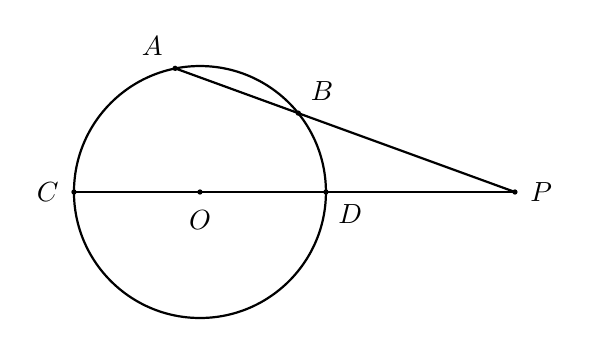
\begin{tikzpicture}[scale=0.8]
  \coordinate (O) at (0,0);
  \coordinate (P) at (5,0);
  \coordinate (C) at (-2,0);
  \coordinate (D) at (2,0);
  \coordinate (B) at (1.561,1.252);
  \coordinate (A) at (-0.394,1.963);
  \draw[thick] (0,0) circle (2);
  \draw[thick] (C)--(P);
  \draw[thick] (P)--(A);
  \fill (O) circle (1.2pt) node[below=3pt] {$O$};
  \fill (P) circle (1.2pt) node[right=2pt] {$P$};
  \fill (C) circle (1.2pt) node[left=2pt] {$C$};
  \fill (D) circle (1.2pt) node[below right=1pt] {$D$};
  \fill (B) circle (1.2pt) node[above right=1pt] {$B$};
  \fill (A) circle (1.2pt) node[above left=1pt] {$A$};
\end{tikzpicture}
\end{center}
\nopagebreak[4]
（1） 试证：$PA\cdot PB=PC\cdot PD$；

（2） 已知：$\odot O$ 的半径为 $1$，$PO=2$，$AB=1$，求 $PA$ 的长。

\Needspace{4\baselineskip}
\textbf{解析}
\nopagebreak[4]
\begin{center}% 1977 年江苏常州市初试卷第 10 题：圆 O 与两条割线——过圆心的割线 P-D-O-C，
% 圆外一点 P 的割线 P-B-A（按源卷第 2 页布局）
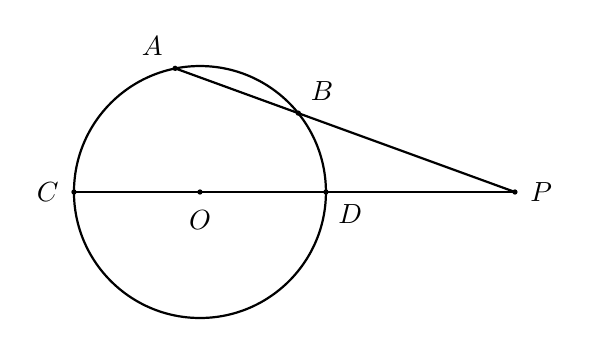
\begin{tikzpicture}[scale=0.8]
  \coordinate (O) at (0,0);
  \coordinate (P) at (5,0);
  \coordinate (C) at (-2,0);
  \coordinate (D) at (2,0);
  \coordinate (B) at (1.561,1.252);
  \coordinate (A) at (-0.394,1.963);
  \draw[thick] (0,0) circle (2);
  \draw[thick] (C)--(P);
  \draw[thick] (P)--(A);
  \fill (O) circle (1.2pt) node[below=3pt] {$O$};
  \fill (P) circle (1.2pt) node[right=2pt] {$P$};
  \fill (C) circle (1.2pt) node[left=2pt] {$C$};
  \fill (D) circle (1.2pt) node[below right=1pt] {$D$};
  \fill (B) circle (1.2pt) node[above right=1pt] {$B$};
  \fill (A) circle (1.2pt) node[above left=1pt] {$A$};
\end{tikzpicture}
\end{center}
\nopagebreak[4]
\gksubpart{（1）}

\Needspace{5\baselineskip}
连接 $AD$、$BC$。在 $\triangle PAD$ 与 $\triangle PCB$ 中：$\angle APD=\angle CPB$（同一角），$\angle PDA=\angle PBC$（同弧 $\overset{\frown}{AC}$ 上的圆周角相等），所以

\nopagebreak[4]
\[
\triangle PAD\sim\triangle PCB
\quad\Longrightarrow\quad
\frac{PA}{PC}=\frac{PD}{PB},
\]

\Needspace{5\baselineskip}
即

\nopagebreak[4]
\[
PA\cdot PB=PC\cdot PD.
\]

\gksubpart{（2）}

\Needspace{5\baselineskip}
$P$ 在圆外，$PO=2$，半径为 $1$，故

\nopagebreak[4]
\[
PC=PO+OC=3,\qquad PD=PO-OD=1,
\]

\Needspace{5\baselineskip}
由（1）得 $PA\cdot PB=PC\cdot PD=3$。又 $A$ 比 $B$ 离 $P$ 远，$PA-PB=AB=1$。设 $PB=t$，则 $PA=t+1$，

\nopagebreak[4]
\[
t(t+1)=3
\quad\Longrightarrow\quad
t^2+t-3=0
\quad\Longrightarrow\quad
t=\frac{-1+\sqrt{13}}{2}\ (\text{\text{负根舍去}}),
\]

\Needspace{5\baselineskip}
所以

\nopagebreak[4]
\[
PA=t+1=\frac{1+\sqrt{13}}{2}.
\]

\gkanswer{答案（1）：见解析版}

\gkanswer{答案（2）：$PA=\dfrac{1+\sqrt{13}}{2}$。}

\end{answer}
\begin{answer}
\gksolhead{11}{}

\textbf{题目}（8 分）：

右图是某物体的二视图，按 $1:1$ 的比例画出这个物体的直观图，并计算它的侧面积。
\nopagebreak[4]
\begin{center}% 1977 年江苏常州市初试卷第 11 题：物体二视图——正视图（底 24 高 16 的三角形）在上，
% 俯视图（24x24 带对角线的正方形）在下，含中心线与尺寸标注（按源卷第 2 页布局）
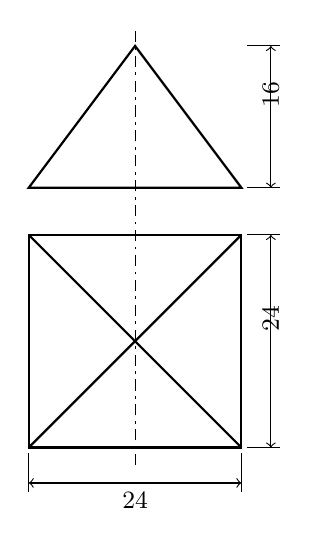
\begin{tikzpicture}[scale=0.75, font=\small]
  % 正视图：三角形
  \draw[thick] (-1.8,2.4)--(1.8,2.4)--(0,4.8)--cycle;
  % 俯视图：正方形与对角线
  \draw[thick] (-1.8,1.6)--(1.8,1.6)--(1.8,-2.0)--(-1.8,-2.0)--cycle;
  \draw[thick] (-1.8,1.6)--(1.8,-2.0);
  \draw[thick] (1.8,1.6)--(-1.8,-2.0);
  % 中心线（点划线）
  \draw[dash pattern=on 4pt off 2pt on 1pt off 2pt] (0,-2.3)--(0,5.1);
  % 尺寸标注引出线
  \draw[thin] (1.9,2.4)--(2.45,2.4);
  \draw[thin] (1.9,4.8)--(2.45,4.8);
  \draw[thin] (1.9,1.6)--(2.45,1.6);
  \draw[thin] (1.9,-2.0)--(2.45,-2.0);
  \draw[thin] (-1.8,-2.1)--(-1.8,-2.75);
  \draw[thin] (1.8,-2.1)--(1.8,-2.75);
  % 尺寸：16（正视图高）
  \draw[<->] (2.3,2.4)--(2.3,4.8) node[midway, right, rotate=90] {$16$};
  % 尺寸：24（俯视图宽）
  \draw[<->] (2.3,-2.0)--(2.3,1.6) node[midway, right, rotate=90] {$24$};
  % 尺寸：24（俯视图长）
  \draw[<->] (-1.8,-2.6)--(1.8,-2.6) node[midway, below] {$24$};
\end{tikzpicture}
\end{center}
\nopagebreak[4]
\Needspace{4\baselineskip}
\textbf{解析}
\nopagebreak[4]
\begin{center}% 1977 年江苏常州市初试卷第 11 题：物体二视图——正视图（底 24 高 16 的三角形）在上，
% 俯视图（24x24 带对角线的正方形）在下，含中心线与尺寸标注（按源卷第 2 页布局）
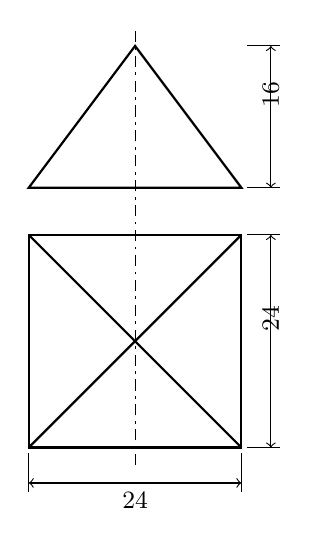
\begin{tikzpicture}[scale=0.75, font=\small]
  % 正视图：三角形
  \draw[thick] (-1.8,2.4)--(1.8,2.4)--(0,4.8)--cycle;
  % 俯视图：正方形与对角线
  \draw[thick] (-1.8,1.6)--(1.8,1.6)--(1.8,-2.0)--(-1.8,-2.0)--cycle;
  \draw[thick] (-1.8,1.6)--(1.8,-2.0);
  \draw[thick] (1.8,1.6)--(-1.8,-2.0);
  % 中心线（点划线）
  \draw[dash pattern=on 4pt off 2pt on 1pt off 2pt] (0,-2.3)--(0,5.1);
  % 尺寸标注引出线
  \draw[thin] (1.9,2.4)--(2.45,2.4);
  \draw[thin] (1.9,4.8)--(2.45,4.8);
  \draw[thin] (1.9,1.6)--(2.45,1.6);
  \draw[thin] (1.9,-2.0)--(2.45,-2.0);
  \draw[thin] (-1.8,-2.1)--(-1.8,-2.75);
  \draw[thin] (1.8,-2.1)--(1.8,-2.75);
  % 尺寸：16（正视图高）
  \draw[<->] (2.3,2.4)--(2.3,4.8) node[midway, right, rotate=90] {$16$};
  % 尺寸：24（俯视图宽）
  \draw[<->] (2.3,-2.0)--(2.3,1.6) node[midway, right, rotate=90] {$24$};
  % 尺寸：24（俯视图长）
  \draw[<->] (-1.8,-2.6)--(1.8,-2.6) node[midway, below] {$24$};
\end{tikzpicture}
\end{center}
\nopagebreak[4]
由二视图：俯视图是边长 $24$ 的正方形且两条对角线方向可见棱，正视图是底 $24$、高 $16$ 的三角形，故该物体是底面边长 $24$、高 $16$ 的正四棱锥，顶点在底面中心正上方。

直观图作法：按 $1:1$ 画出底面正方形及其对角线，取对角线交点，在其正上方高 $16$ 处定顶点，连四条侧棱。

\Needspace{5\baselineskip}
侧面三角形的高（斜高）

\nopagebreak[4]
\[
h'=\sqrt{16^2+12^2}=\sqrt{256+144}=20,
\]

\Needspace{5\baselineskip}
侧面积

\nopagebreak[4]
\[
S=4\times\frac{1}{2}\times24\times20=960.
\]

\gkanswer{答案：侧面积为 $960$。}

\end{answer}
\begin{answer}
\gksolhead{12}{}

\textbf{题目}（8 分）：

已知：三点 $A(-2,\ 9)$，$B(4,\ -4)$，$C(10,\ 8)$．试求：

（1） 过 $A$ 点且垂直于 $BC$ 的直线方程；

（2） $A$ 点到 $BC$ 的距离。

\Needspace{4\baselineskip}
\textbf{解析}

\gksubpart{（1）}

\Needspace{5\baselineskip}
$BC$ 的斜率

\nopagebreak[4]
\[
k_{BC}=\frac{8-(-4)}{10-4}=2.
\]

\Needspace{5\baselineskip}
所求直线过 $A(-2,\ 9)$ 且与 $BC$ 垂直，斜率为 $-\dfrac{1}{2}$：

\nopagebreak[4]
\[
y-9=-\frac{1}{2}(x+2)
\quad\Longrightarrow\quad
x+2y-16=0.
\]

\gksubpart{（2）}

\Needspace{5\baselineskip}
$BC$ 所在直线为 $y+4=2(x-4)$，即 $2x-y-12=0$。$A$ 点到 $BC$ 的距离

\nopagebreak[4]
\[
d=\frac{|2\times(-2)-9-12|}{\sqrt{2^2+(-1)^2}}=\frac{25}{\sqrt{5}}=5\sqrt{5}.
\]

\gkanswer{答案（1）：$x+2y-16=0$。}

\gkanswer{答案（2）：$5\sqrt{5}$。}

\end{answer}
\begin{answer}
\gksolhead{13}{}

\textbf{题目}（8 分）：

如图：在直角坐标系中，$OA_0=1$，以 $OA_0$ 为一条直角边画出第一个直角三角形 $OA_0A_1$，又以 $OA_1$ 为一直角边画出第二个直角三角形 $OA_1A_2$，再以 $OA_2$ 为一直角边画出第三个直角三角形 $OA_2A_3$，依次继续画下去，试求：
\nopagebreak[4]
\begin{center}% 1977 年江苏常州市初试卷第 13 题：极坐标系中依次旋转 30 度的螺旋直角三角形序列
% OA0A1...A4（Ak 在极角 30k 度的射线上，直角顶点为 Ak），十二 条 30 度间隔射线按原卷标注（按源卷第 3 页布局）
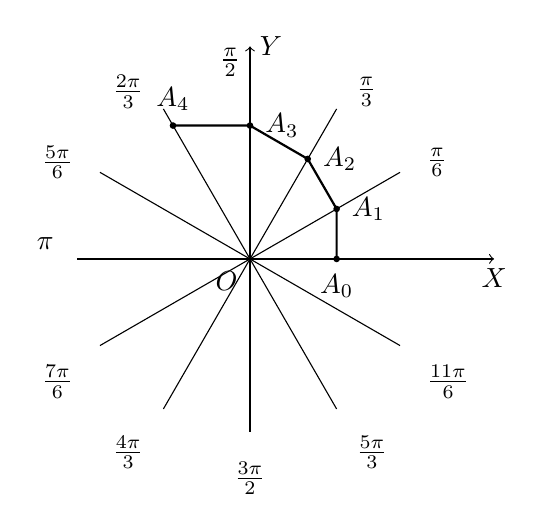
\begin{tikzpicture}[scale=1.0]
  % 十二条 30 度间隔射线
  \foreach \a in {0,30,...,330}{\draw[thin] (0,0)--(\a:2.2);}
  % 坐标轴
  \draw[->, thin] (0,0)--(3.1,0) node[below] {$X$};
  \draw[->, thin] (0,0)--(0,2.7) node[right] {$Y$};
  % 螺旋折线 A0-A1-A2-A3-A4（OA0=1 对应 1.1cm，公比 2/\sqrt{3}）
  \draw[thick] (1.1,0)--(1.1,0.635)--(0.733,1.270)--(0,1.694)--(-0.978,1.694);
  \fill (1.1,0) circle (1.2pt) node[below=2pt] {$A_0$};
  \fill (1.1,0.635) circle (1.2pt) node[right=2pt] {$A_1$};
  \fill (0.733,1.270) circle (1.2pt) node[right=2pt] {$A_2$};
  \fill (0,1.694) circle (1.2pt) node[right=2pt] {$A_3$};
  \fill (-0.978,1.694) circle (1.2pt) node[above=2pt] {$A_4$};
  \node[below left=1pt] at (0,0) {$O$};
  % 射线极角标注
  \node[right] at (30:2.45) {$\frac{\pi}{6}$};
  \node[right] at (60:2.45) {$\frac{\pi}{3}$};
  \node[left] at (90:2.5) {$\frac{\pi}{2}$};
  \node[left] at (120:2.45) {$\frac{2\pi}{3}$};
  \node[left] at (150:2.45) {$\frac{5\pi}{6}$};
  \node[above] at (180:2.6) {$\pi$};
  \node[below left] at (210:2.45) {$\frac{7\pi}{6}$};
  \node[below left] at (240:2.45) {$\frac{4\pi}{3}$};
  \node[below] at (270:2.45) {$\frac{3\pi}{2}$};
  \node[below right] at (300:2.45) {$\frac{5\pi}{3}$};
  \node[below right] at (330:2.45) {$\frac{11\pi}{6}$};
\end{tikzpicture}
\end{center}
\nopagebreak[4]
（1） $A_6$ 点的极坐标；

（2） 第十二个直角三角形的面积（精确到 $0.01$）。

已知 $\lg2=0.3010$，$\lg3=0.4771$。原卷随题印有「反对数表」节选（标准四位反对数表第 80—84 行、第 0—5 列），转录如下：

\begin{center}
\begin{tabular}{lllllll}
\toprule
m & 0 & 1 & 2 & 3 & 4 & 5 \\
\midrule
80 & 6310 & 6324 & 6339 & 6353 & 6368 & 6383 \\
81 & 6457 & 6471 & 6486 & 6501 & 6516 & 6531 \\
82 & 6607 & 6622 & 6637 & 6653 & 6668 & 6683 \\
83 & 6761 & 6776 & 6792 & 6808 & 6823 & 6839 \\
84 & 6918 & 6934 & 6950 & 6966 & 6982 & 6998 \\
\bottomrule
\end{tabular}
\end{center}

\Needspace{4\baselineskip}
\textbf{解析}
\nopagebreak[4]
\begin{center}% 1977 年江苏常州市初试卷第 13 题：极坐标系中依次旋转 30 度的螺旋直角三角形序列
% OA0A1...A4（Ak 在极角 30k 度的射线上，直角顶点为 Ak），十二 条 30 度间隔射线按原卷标注（按源卷第 3 页布局）
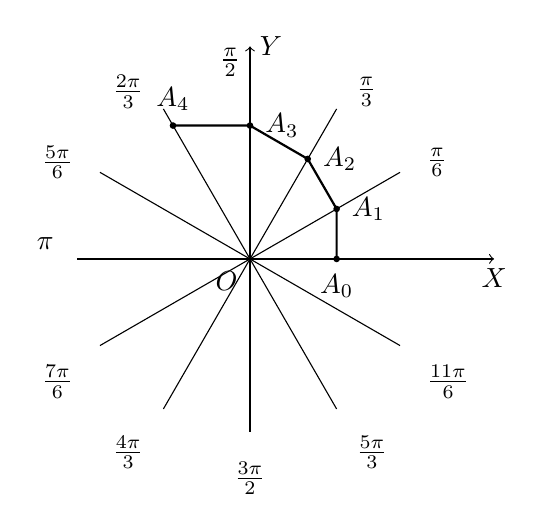
\begin{tikzpicture}[scale=1.0]
  % 十二条 30 度间隔射线
  \foreach \a in {0,30,...,330}{\draw[thin] (0,0)--(\a:2.2);}
  % 坐标轴
  \draw[->, thin] (0,0)--(3.1,0) node[below] {$X$};
  \draw[->, thin] (0,0)--(0,2.7) node[right] {$Y$};
  % 螺旋折线 A0-A1-A2-A3-A4（OA0=1 对应 1.1cm，公比 2/\sqrt{3}）
  \draw[thick] (1.1,0)--(1.1,0.635)--(0.733,1.270)--(0,1.694)--(-0.978,1.694);
  \fill (1.1,0) circle (1.2pt) node[below=2pt] {$A_0$};
  \fill (1.1,0.635) circle (1.2pt) node[right=2pt] {$A_1$};
  \fill (0.733,1.270) circle (1.2pt) node[right=2pt] {$A_2$};
  \fill (0,1.694) circle (1.2pt) node[right=2pt] {$A_3$};
  \fill (-0.978,1.694) circle (1.2pt) node[above=2pt] {$A_4$};
  \node[below left=1pt] at (0,0) {$O$};
  % 射线极角标注
  \node[right] at (30:2.45) {$\frac{\pi}{6}$};
  \node[right] at (60:2.45) {$\frac{\pi}{3}$};
  \node[left] at (90:2.5) {$\frac{\pi}{2}$};
  \node[left] at (120:2.45) {$\frac{2\pi}{3}$};
  \node[left] at (150:2.45) {$\frac{5\pi}{6}$};
  \node[above] at (180:2.6) {$\pi$};
  \node[below left] at (210:2.45) {$\frac{7\pi}{6}$};
  \node[below left] at (240:2.45) {$\frac{4\pi}{3}$};
  \node[below] at (270:2.45) {$\frac{3\pi}{2}$};
  \node[below right] at (300:2.45) {$\frac{5\pi}{3}$};
  \node[below right] at (330:2.45) {$\frac{11\pi}{6}$};
\end{tikzpicture}
\end{center}
\nopagebreak[4]
\Needspace{5\baselineskip}
由图，$A_0$ 在极轴上，$A_1\text{、}A_2\text{、}A_3\text{、}A_4$ 依次落在极角 $30^\circ,60^\circ,90^\circ,120^\circ$ 的射线上，即每个直角三角形在顶点 $O$ 处的锐角都是 $30^\circ$，直角顶点为 $A_k$。于是对每个 $k$，

\nopagebreak[4]
\[
A_kA_{k+1}=OA_k\tan30^\circ,\qquad
OA_{k+1}=\frac{OA_k}{\cos30^\circ}=\frac{2}{\sqrt{3}}\,OA_k,
\]

\Needspace{5\baselineskip}
从而

\nopagebreak[4]
\[
OA_n=\left(\frac{2}{\sqrt{3}}\right)^{n}.
\]

\gksubpart{（1）}

\Needspace{5\baselineskip}
$A_6$ 在极角 $6\times30^\circ=180^\circ$ 即 $\pi$ 的射线上，

\nopagebreak[4]
\[
OA_6=\left(\frac{2}{\sqrt{3}}\right)^{6}=\left(\frac{4}{3}\right)^{3}=\frac{64}{27},
\]

故 $A_6$ 的极坐标为 $\left(\dfrac{64}{27},\ \pi\right)$。

\gksubpart{（2）}

\Needspace{5\baselineskip}
第十二个直角三角形为 $OA_{11}A_{12}$，其面积

\nopagebreak[4]
\[
S_{12}=\frac{1}{2}\,OA_{11}\cdot A_{11}A_{12}
=\frac{1}{2}\,OA_{11}^{2}\tan30^\circ
=\frac{1}{2}\left(\frac{2}{\sqrt{3}}\right)^{22}\cdot\frac{1}{\sqrt{3}}
=\frac{2^{21}}{3^{11}\sqrt{3}}.
\]

\Needspace{5\baselineskip}
两边取常用对数（用原卷给定的 $\lg2=0.3010$、$\lg3=0.4771$）：

\nopagebreak[4]
\[
\lg S_{12}=21\lg2-\left(11+\frac{1}{2}\right)\lg3
=21\times0.3010-11.5\times0.4771
=6.3210-5.4867=0.8344.
\]

\Needspace{5\baselineskip}
查原卷反对数表：首数 $0$、尾数 $0.8344$，第 83 行第 4 列为 $6823$，内插第 5 列 $6839$ 得 $10^{0.8344}\approx6.83$，所以

\nopagebreak[4]
\[
S_{12}\approx6.83.
\]

（按精确值复核：$S_{12}=\dfrac{2^{21}}{3^{11}\sqrt{3}}\approx6.83$，与查表一致。）

\gkanswer{答案（1）：$A_6\left(\dfrac{64}{27},\ \pi\right)$。}

\gkanswer{答案（2）：约 $6.83$。}

\end{answer}